% %
% % Insert title of manuscript and other info on comment lines here
% %
% % REVTEX 3.0 source file.  Format using the Latex program.
% % REVTEX style files (aps.sty, etc) must be installed on the system.
% % REVTEX is supported by the American Institute of Physics (AIP)
% % The appropriate format for Journal of Chemical Physics is Phys. Rev. B
% %   (option ``prb'' in documentstyle).  Documentstyle option ``preprint''
% %   gives larger font.
% %
% 
% % David's preamble
% \date{\today}
% 
% %\documentclass[journal=jacsat,manuscript=communication,layout=twocolumn]{achemso}
% %\documentclass[jctcce,letterpaper,twocolumn,floatfix,preprintnumbers,superscriptaddress]{revtex4}
% % \documentclass[12pt,preprint,aps,prb]{revtex4}
% % \documentclass[aps,preprint,showpacs,superscriptaddress,groupedaddress]{revtex4}  % for double-spaced preprint
% \documentclass[aps,prl,twocolumn,superscriptaddress,groupedaddress]{revtex4}  % for review and submission
% \usepackage{dcolumn,graphicx,amsmath,amssymb,algorithm,algpseudocode}
% \usepackage{todonotes}
% \usepackage{qcircuit}
% 
% \newcommand{\ud}{\mathrm{d}}
% \newcommand{\erf}{\mathrm{erf}}
% \newcommand{\erfc}{\mathrm{erfc}}
% \newcommand{\diff}[2]{\frac{\ud {#1}}{\ud {#2}}}
% \newcommand{\pdiff}[2]{\frac{\partial #1}{\partial #2}}
% 
% \begin{document}
% 
% 
% \title{
% Supplemental Material for: 
% Quantum Computation of Electronic Transitions using a Variational Quantum
% Eigensolver
% }
% 
% \author{Robert M. Parrish}
% \affiliation{
% Department of Chemistry and the PULSE Institute, Stanford University, Stanford, CA 94305
%     }
% \affiliation{
% SLAC National Accelerator Laboratory, Menlo Park, CA 94025
% }
% \affiliation{
% QC Ware Corporation,  Palo Alto, CA 94301
% }
% 
% \author{Edward G. Hohenstein}
% \affiliation{
% Department of Chemistry and the PULSE Institute, Stanford University, Stanford, CA 94305
%     }
% \affiliation{
% SLAC National Accelerator Laboratory, Menlo Park, CA 94025
% }
% 
% \author{Peter L. McMahon}
% \affiliation{
% E.\,L.~Ginzton Laboratory, Stanford University, Stanford, CA 94305
%     }
% \affiliation{
% QC Ware Corporation,  Palo Alto, CA 94301
% }
% 
% \author{Todd J. Mart\'inez}
% \affiliation{
% Department of Chemistry and the PULSE Institute, Stanford University, Stanford, CA 94305
%     }
% \affiliation{
% SLAC National Accelerator Laboratory, Menlo Park, CA 94025
% }
% \email{Todd.Martinez@gmail.com}
% 
% \maketitle

\section{Supplemental Material}

\section{Hamiltonian Manipulation}

Consider an \emph{ab initio} exciton model of $N$ chromophoric monomers labelled
by index $A$, each with two monomer electronic states labeled $|0_A\rangle$
(ground) and $|1_A\rangle$ (excited). The \emph{ab initio} exciton Hamiltonian
is
\begin{equation}
\label{eq:H}
\hat H
=
\hat H^{(1)}
+
\hat H^{(2)}
\end{equation}
\[
=
\sum_{A}
\sum_{p,q \in 0,1}
(p_{A} | \hat h | q_{A})
| p_{A} \rangle
\langle q_{A} |
\]
\[
+
\sum_{A>B}
\sum_{p,q,r,s \in 0,1}
(p_{A} q_{A} | \hat v | r_{B} s_{B})
|p_{A} \rangle
\langle q_{A} |
\otimes
|r_{B} \rangle
\langle s_{B} |
\]
The real one-body matrix elements $(p_A|\hat h|q_A)$ are usually the 
(diagonal) adiabatic energy levels of the ground and first excited state of the
isolated monomers, while the real two-body matrix elements $(p_A q_A|\hat v|r_B
s_B)$ are the electrostatic interactions between the one-body densities (e.g.,
for $p = q$) or one-body transition densities (e.g., for $p \neq q$) of monomers
$A$ and $B$.  These matrix elements can be computed accurately with polynomial
cost (albeit expensive in absolute/prefactor considerations and requiring
extensive efforts to accelerate) by \emph{ab initio} electronic structure
computations performed on classical computers, for monomers with at least
several hundred atoms. 

\textbf{Pauli Operator Notation:} The one-body operator is,
\begin{equation}
\hat H^{(1)}
=
\sum_{A}
(0_A | \hat h | 0_A) | 0_A \rangle \langle 0_A |
+
(1_A | \hat h | 1_A) | 1_A \rangle \langle 1_A |
\end{equation}
\[
+
(0_A | \hat h | 1_A) | 0_A \rangle \langle 1_A |
+
(1_A | \hat h | 0_A) | 1_A \rangle \langle 0_A |
\]
\[
=
\sum_{A}
\frac{(0_A|\hat h|0_A) + (1_A|\hat h|1_A)}{2} \hat I_{A}
\]
\[
+
\frac{(0_A|\hat h|0_A) - (1_A|\hat h|1_A)}{2} \hat Z_{A}
\]
\[
+ (0_A|\hat h|1_A) \hat X_{A}
\]
\[
\equiv
\sum_{A}
S_A \hat I_{A}
+
D_A \hat Z_{A}
+
X_A \hat X_{A}
\]
Here $S_{A} = [(0_A | \hat h | 0_A) +
(1_A | \hat h | 1_A)] / 2$, $D_{A} \equiv [(0_A | \hat h | 0_A) - (1_A | \hat h
| 1_A)] / 2$, and $X_{A} = (0_A | \hat h | 1_A)$. When switching to Pauli matrix
notation on the second line, we use the implicit convention that any matrices
not shown are taken to be the identity, e.g., $\hat Z_{C} \equiv \hat I_{A}
\otimes \hat I_{B} \otimes \hat Z_{C} \otimes I_{D} \otimes \ldots \otimes \hat
I_{N}$. Note that the off-diagonal intramonomer couplings $X_A = (0_A | \hat h |
1_A)$ are usually defined to be zero in our exciton model convention, but there
is no overhead for including them here (there will be another $\hat X_A$ gate
contribution below).

The two-body operator $\hat H^{(2)}$ requires a bit more work to convert to a
form containing only sums of tensor products of Pauli operators. For each
two-body term,
\begin{equation}
H_{AB}
=
\end{equation}
\[
  (H_A | H_B) \hat H_A \otimes \hat H_B
+ (H_A | T_B) \hat H_A \otimes \hat X_B
\]
\[
+ (T_A | H_B) \hat X_A \otimes \hat H_B
+ (T_A | T_B) \hat X_A \otimes \hat X_B
\]
\[
+ (H_A | P_B) \hat H_A \otimes \hat P_B
+ (P_A | H_B) \hat P_A \otimes \hat H_B
\]
\[
+ (T_A | P_B) \hat X_A \otimes \hat P_B
+ (P_A | T_B) \hat P_A \otimes \hat X_B
\]
\[
+ (P_A | P_B) \hat P_A \otimes \hat P_B
\]
Here $H$, $P$, and $T$ represent ``hole,'' ``particle,'' and ``transition,''
respectively. $\hat H \equiv [\hat I + \hat Z] / 2$ and $\hat P \equiv [\hat I
- \hat Z] / 2$ are the hole and particle counting operators, respectively. Note
  that $\hat I = \hat H + \hat P$ and $\hat Z = \hat H - \hat P$ The two-body
matrix elements are,
\begin{equation}
(H_A | H_B) 
=
(0_A 0_A | \hat v | 0_B 0_B)
\end{equation}
\begin{equation}
(H_A | T_B) 
=
(0_A 0_A | \hat v | 0_B 1_B)
=
(0_A 0_A | \hat v | 1_B 0_B)
\end{equation}
\begin{equation}
(H_A | P_B)
=
(0_A 0_A | \hat v | 1_B 1_B)
\end{equation}
and so forth.

Terms 2, 3, 7, and 8 above can be written as,
\begin{equation}
+ (H_A | T_B) \hat H_A \otimes \hat X_B
+ (T_A | H_B) \hat X_A \otimes \hat H_B
\end{equation}
\[
+ (T_A | P_B) \hat X_A \otimes \hat P_B
+ (P_A | T_B) \hat P_A \otimes \hat X_B
\]
\[
=
  (S_A | T_B) \hat I_A \otimes X_B
+ (D_A | T_B) \hat Z_A \otimes X_B
\]
\[
=
+ (T_A | S_B) \hat X_A \otimes I_B
+ (T_A | D_B) \hat X_A \otimes Z_B
\]

Terms 1, 5, 6, and 9 above can be written as,
\begin{equation}
  (H_A | H_B) \hat H_A \otimes \hat H_B
+ (H_A | P_B) \hat H_A \otimes \hat P_B
\end{equation}
\[
+ (P_A | H_B) \hat P_A \otimes \hat H_B
+ (P_A | P_B) \hat P_A \otimes \hat P_B
\]
\[
=
  (S_A | S_B) \hat I_A \otimes \hat I_B
+ (S_A | D_B) \hat I_A \otimes \hat Z_B
\]
\[
+ (D_A | S_B) \hat Z_A \otimes \hat I_B
+ (D_A | D_A) \hat Z_A \otimes \hat Z_B
\]

In the above,
\begin{equation}
(S_A | T_B) = (H_A + P_A | T_B) / 2 
\end{equation}
\[
= [(H_A | T_B) + (P_A | T_B)] / 2
\]
\begin{equation}
(D_A | T_B) = (H_A - P_A | T_B) / 2 
\end{equation}
\[
= (H_A | T_B) - [(P_A | T_B)] / 2
\]
and so forth.

So the two-body Hamiltonian element can be written as,
\begin{equation}
\hat H_{AB}^{(2)} = 
   (S_A | S_B) \hat I_A \otimes \hat I_B
\end{equation}
\[
+  (S_A | D_B) \hat I_A \otimes \hat Z_B
+  (D_A | S_A) \hat Z_A \otimes \hat I_B
\]
\[
+  (S_A | T_B) \hat I_A \otimes \hat X_B
+  (T_A | S_A) \hat X_A \otimes \hat I_B
\]
\[
+  (T_A | T_B) \hat X_A \otimes \hat X_B
+  (T_A | D_B) \hat X_A \otimes \hat Z_B
\]
\[
+  (D_A | T_B) \hat Z_A \otimes \hat X_B
+  (D_A | D_B) \hat Z_A \otimes \hat Z_B
\]


\textbf{Hamiltonian in Pauli Notation:} After the straightforward
algebra above, the total Hamiltonian can be written as,
\begin{equation}
\label{eq:H_N}
\hat H
=
\mathcal{E}
+
\mathcal{H}^{(1)}
+
\mathcal{H}^{(2)}
=
\mathcal{E} \hat I 
+ 
\sum_{A}
\mathcal{Z}_{A}
\hat Z_{A}
+
\mathcal{X}_{A}
\hat X_{A}
\end{equation}
\[
+
\sum_{A > B}
\mathcal{XX}_{AB}
\hat X_{A} \otimes \hat X_{B}
+
\mathcal{XZ}_{AB}
\hat X_{A} \otimes \hat Z_{B}
\]
\[
+
\mathcal{ZX}_{AB}
\hat Z_{A} \otimes \hat X_{B}
+
\mathcal{ZZ}_{AB}
\hat Z_{A} \otimes \hat Z_{B}
\]
The matrix elements are,
\begin{equation}
\mathcal{E}
=
\sum_{A}
S_{A}
+
\sum_{A>B}
(S_A | S_B)
\end{equation}
\begin{equation}
\mathcal{Z}_{A}
=
D_{A}
+
\sum_{B}
(D_{A} | S_{B})
\end{equation}
\begin{equation}
\mathcal{X}_{A} 
=
X_{A}
+
\sum_{B}
(T_{A} | S_{B})
\end{equation}
\begin{equation}
\mathcal{XX}_{AB}
=
(T_{A} | T_{B})
\end{equation}
\begin{equation}
\mathcal{XZ}_{AB}
=
(T_{A} | D_{B})
\end{equation}
\begin{equation}
\mathcal{ZX}_{AB}
=
(D_{A} | T_{B})
\end{equation}
\begin{equation}
\mathcal{ZZ}_{AB}
=
(D_{A} | D_{B})
\end{equation}
More specifically,
\begin{equation}
S_{A} = 
\left [
(0_A | \hat h |0_A)
+
(1_A | \hat h |1_A)
\right ] / 2
\end{equation}
\begin{equation}
D_{A} = 
\left [
(0_A | \hat h |0_A)
-
(1_A | \hat h |1_A)
\right ] / 2
\end{equation}
\begin{equation}
X_{A} =
(0_A | \hat h | 1_A)
\end{equation}
\begin{equation}
(T_A | T_B) 
=
(0_A 1_A | \hat v | 0_B 1_B)
\end{equation}
\begin{equation}
(T_A | S_B) 
=
(0_A 1_A | \hat v | 0_B 0_B + 1_B 1_B) / 2
\end{equation}
\begin{equation}
(T_A | D_B) 
=
(0_A 1_A | \hat v | 0_B 0_B - 1_B 1_B) / 2
\end{equation}
\begin{equation}
(S_A | T_B) 
=
(0_A 0_A + 1_A 1_A | \hat v | 0_B 1_B) / 2
\end{equation}
\begin{equation}
(D_A | T_B) 
=
(0_A 0_A - 1_A 1_A | \hat v | 0_B 1_B) / 2
\end{equation}
\begin{equation}
(S_A | S_B)
=
(0_A 0_A + 1_A 1_A | \hat v | 0_B 0_B + 1_B 1_B) / 4
\end{equation}
\begin{equation}
(S_A | D_B)
=
(0_A 0_A + 1_A 1_A | \hat v | 0_B 0_B - 1_B 1_B) / 4
\end{equation}
\begin{equation}
(D_A | S_B)
=
(0_A 0_A - 1_A 1_A | \hat v | 0_A 0_B + 1_A 1_B) / 4
\end{equation}
\begin{equation}
(D_A | D_B)
=
(0_A 0_A - 1_A 1_A | \hat v | 0_A 0_B - 1_A 1_B) / 4
\end{equation}
Note that $\{ \mathcal{Z}_{A} \}$ are expected to be the largest matrix elements
in this Hamiltonian, and are of the order of a few eV ($10^{-2} - 10^{-1}$ au).
In practice, we typically find the $\{ \mathcal{X}_{A} \}$ and $\{
\mathcal{XX}_{AB} \}$ are the next largest matrix elements ($10^{-3} - 10^{-2}$
au). These are rough estimates which may differ in specific systems.

\section{MC-VQE Technical Details}

\textbf{CIS State Preparation:} An important task for excited state MC-VQE is to
prepare the configuration interaction singles (CIS) state,
\[
| \Phi_{\Theta} \rangle
\equiv
\mu | 000 \ldots \rangle
+
\alpha | 100\ldots \rangle
+
\beta | 010\ldots \rangle
+
\gamma | 001\ldots \rangle
+
\ldots
\]
\begin{equation}
:
\sqrt{
\mu^2
+
\alpha^2
+
\beta^2
+
\gamma^2
\ldots
}
=
1
\end{equation}
The parameters $\mu, \alpha, \beta, \gamma \ldots$ are obtained classically by
solving the CIS eigenproblem. Note that the CIS eigenstates are definitionally
orthonormal,
\begin{equation}
\langle \Phi_{\Theta} | \Phi_{\Theta'} \rangle
=
\delta_{\Theta, \Theta'}
, \
\Theta, \Theta' \in [0, N]
\end{equation}
Note that there are $N+1$ states in the CIS manifold used in this work: $1$ for
the reference ground configuration ($|000 \ldots \rangle$) and $N$ for the
singly-excited configurations ($|100 \ldots \rangle$ and so forth), all of which
are allowed to mix in our CIS prescription.

A circuit to prepare the CIS state is sketched for $N=5$,
\begin{widetext}
\begin{equation}
\Qcircuit @R=1.0em @C=1.0em {
\lstick{|0_A\rangle}
 & \gate{R_{y} (\theta_0)}
 & \ctrl{1}
 & \qw
 & \qw
 & \qw
 & \qw
 & \qw
 & \qw
 & \qw
 & \qw
 & \qw
 & \targ
 & \targ
 & \targ
 & \targ
 & \qw \\
\lstick{|0_B\rangle}
 & \qw
 & \gate{F_{y} (\theta_{AB}) }
 & \ctrl{1}
 & \qw
 & \qw
 & \qw
 & \qw
 & \qw
 & \targ
 & \targ
 & \targ
 & \qw
 & \qw
 & \qw
 & \ctrl{-1}
 & \qw \\
\lstick{|0_C\rangle}
 & \qw
 & \qw
 & \gate{F_{y} (\theta_{BC}) }
 & \ctrl{1}
 & \qw
 & \qw
 & \targ
 & \targ
 & \qw
 & \qw
 & \ctrl{-1}
 & \qw
 & \qw
 & \ctrl{-2}
 & \qw
 & \qw \\
\lstick{|0_D\rangle}
 & \qw
 & \qw
 & \qw
 & \gate{F_{y} (\theta_{CD}) }
 & \ctrl{1}
 & \targ
 & \qw
 & \ctrl{-1}
 & \qw
 & \ctrl{-2}
 & \qw
 & \qw
 & \ctrl{-3}
 & \qw
 & \qw
 & \qw \\
\lstick{|0_E\rangle}
 & \qw
 & \qw
 & \qw
 & \qw
 & \gate{F_{y} (\theta_{DE}) }
 & \ctrl{-1}
 & \ctrl{-2}
 & \qw
 & \ctrl{-3}
 & \qw
 & \qw
 & \ctrl{-4}
 & \qw
 & \qw
 & \qw
 & \qw 
% \gategroup{3}{5}{5}{7}{0.7em}{--}
\\
}
\end{equation}
\end{widetext}
The $R_y (\Theta_0)$ ``pump'' gate always goes with $|0_A\rangle$, otherwise the
circuit nests ``matryoshka'' style.

The controlled $F_y (\theta)$ gate is,
\begin{widetext}
\begin{equation}
\Qcircuit @R=1.0em @C=1.0em {
& \ctrl{1} & \qw  \\
& \gate{F_{y} (\theta)} & \qw \\
}
=
\Qcircuit @R=1.0em @C=1.0em {
& \qw & \ctrl{1} & \qw & \qw  \\
& \gate{R_{y} (-\theta/2)} & \gate{Z} & \gate{R_{y} (+\theta/2)} & \qw \\
}
=
\Qcircuit @R=1.0em @C=1.0em {
& \qw & \qw & \ctrl{1} & \qw & \qw & \qw  \\
& \gate{R_{y} (-\theta/2)} & \gate{H} & \targ & \gate{H} & \gate{R_{y} (+\theta/2)} & \qw \\
}
=
\left [
\begin{array}{cccc}
 1 & & & \\
 & 1 & & \\
 & & +c(\theta) & +s(\theta) \\
 & & +s(\theta) & -c(\theta) \\
\end{array}
\right ]
\end{equation}
\end{widetext}

By inspection,
\begin{equation}
\mu
=
\cos \theta_{0}
\end{equation}
\begin{equation}
\alpha
=
\sin \theta_{0}
\cos \theta_{AB}
\end{equation}
\begin{equation}
\beta
=
\sin \theta_{0}
\sin \theta_{AB}
\cos \theta_{BC}
\end{equation}
\begin{equation}
\gamma
=
\sin \theta_{0}
\sin \theta_{AB}
\sin \theta_{BC}
\cos \theta_{CD}
\end{equation}
\begin{equation}
\vdots
\end{equation}
\begin{equation}
\eta
=
\sin \theta_{0}
\ldots
\sin \theta_{LM}
\sin \theta_{MN}
\end{equation}
Thus we can evaluate the angles recursively,
\begin{equation}
\theta_{0}
=
\cos^{-1} (\mu)
\end{equation}
\begin{equation}
\theta_{AB}
=
\cos^{-1} (\alpha / (\sin(\theta_{0})))
\end{equation}
\begin{equation}
\theta_{BC}
=
\cos^{-1} (\beta / (\sin(\theta_{0}) \sin(\theta_{AB})))
\end{equation}
\begin{equation}
\theta_{CD}
=
\cos^{-1} (\gamma / (\sin(\theta_{0}) \sin(\theta_{AB}) \sin(\theta_{BC})))
\end{equation}
\begin{equation}
\vdots
\end{equation}
\begin{equation}
\theta_{MN}
=
\cos^{-1} (\mu / (\sin(\theta_{0}) \sin(\theta_{AB}) \sin(\theta_{BC}) \ldots \sin(\theta_{LM})))
\end{equation}
Note that the last angle $\theta_{MN}$ is only resolved up to a phase factor of
$\pm 1$: the explicit value of $\eta$ must be checked using the last line of the
forward formula above to determine the phase factor (the relative error will be
0 [+1] or 2 [-1], which makes the check particularly easy).

The ``interference'' state $(|\Phi_{\Theta}\rangle \pm | \Phi_{\Theta'} \rangle)
/ \sqrt{2}$ can easily be formed by substitutions of the coefficients
\begin{equation}
\mu^{\pm}
=
(
\mu^{\Theta}
\pm
\mu^{\Theta'}
) / \sqrt{2}
\end{equation}
\begin{equation}
\alpha^{\pm}
=
(
\alpha^{\Theta}
\pm
\alpha^{\Theta'}
) / \sqrt{2}
\end{equation}
\begin{equation}
\vdots
\end{equation}

Note that the CIS state with $\mu = 0, \alpha = \beta = \gamma = \ldots = 1 /
\sqrt{N}$ is usually called the $|W_N\rangle$ state. A circuit for the $|W_N
\rangle$ that was used as the basis for this work is presented in
\cite{Diker:2016:W}.

\textbf{VQE Global Entangler Matrix:} In any configuration-space basis, the
adiabatic eigenfunctions of the real electronic or \emph{ab initio} exciton
Hamiltonian can be written as real, orthonormal vectors with arbitrary total
phase of $\pm 1$. Therefore, the VQE entangler operator $\hat U$ can be
restricted to $SO(2^N)$ without loss.  We have elected to construct the total VQE
entangler circuit for the \emph{ab initio} exciton model by placing a two-body
entangler restricted to $SO(4)$ at each two-body interaction site in the exciton
Hamiltonian. E.g., for a linear arrangement,
\begin{widetext}
\begin{equation}
\label{eq:vqe-top}
\Qcircuit @R=1.0em @C=1.0em {
\lstick{| A \rangle}
& \multigate{1}{U_{2}^{AB}}
& \qw
& \qw \\
\lstick{| B \rangle}
& \ghost{U_{2}^{AB}}
& \multigate{1}{U_{2}^{BN}}
& \qw \\
\lstick{| N \rangle}
& \multigate{1}{U_{2}^{NZ}}
& \ghost{U_{2}^{BN}}
& \qw \\
\lstick{| Z \rangle}
& \ghost{U_{2}^{NZ}}
& \qw
& \qw \\
}
\end{equation}
\end{widetext}
If additional variational flexibility in the ansatz is desired, a
straightforward approach is to add additional layers of entanglers of the form
shown here, or to extend two-body entanglers to the next layer(s) of nearest
neighbors.

Details of the specific VQE two-body entangler $\hat U_2$ restricted to $SO(4)$
that is used in this work are presented below - these manipulations are intended
to produce a VQE two-body entangler whose parameters are easy to guess (e.g.,
starting from all zeros) and to optimize with partial gradient information
(e.g., by simple gradient-descent or L-BFGS) for problems encountered in the
\emph{ab initio} exciton model.

Note that there has been much interest in the literature on the construction of
optimal 2-body quantum circuits covering $SU(4)$ or $SO(4)$ using various or
arbitrary gate libraries - for an overview, see
\cite{Zhang:2003:027903,Shende:2004:062321,Vatan:2004:032315,Wei:2012:X}. 

\textbf{VQE Two-Body Entangler Matrix:} $SO(4)$ is the group of real, orthogonal
matrices with determinant $+1$, and covers all possible two-body entangler
matrices needed in our VQE task. There are infinitely many equivalent logical
parametrizations of $SO(4)$ with 6 real parameters, but some of these will prove
easier to optimize than others in VQE applications. 

For instance, one particularly straightforward parametrization of $SO(4)$ is
given by,
\begin{equation}
\label{eq:so4mark1}
\hat U_2
=
\exp
\left (
\left [
\begin{array}{cccc}
 0 & +A & +B & +C \\
-A &  0 & +D & +E \\
-B & -D &  0 & +F \\
-C & -E & -F &  0 \\
\end{array}
\right ]
\right )
\end{equation}
That is, any special orthogonal matrix for $N=4$ can be written as the matrix
exponential of an $N=4$ antisymmetric matrix with 6 unconstrained real
parameters $A$ through $F$.

Another, equivalent parametrization can be realized by considering the two-body
Pauli generators of the antisymmetric group,
\begin{equation}
-i \hat Y_{A} \otimes \hat I_{B}
=
\left [
\begin{array}{cccc}
 0 &  0 & -1 &  0 \\
 0 &  0 &  0 & -1 \\
+1 &  0 &  0 &  0 \\
 0 & +1 &  0 &  0 \\
\end{array}
\right ]
\end{equation}
\begin{equation}
-i \hat Y_{A} \otimes \hat X_{B}
=
\left [
\begin{array}{cccc}
 0 &  0 &  0 & -1 \\
 0 &  0 & -1 &  0 \\
 0 & +1 &  0 &  0 \\
+1 &  0 &  0 &  0 \\
\end{array}
\right ]
\end{equation}
\begin{equation}
-i \hat Y_{A} \otimes \hat Z_{B}
=
\left [
\begin{array}{cccc}
 0 &  0 & -1 &  0 \\
 0 &  0 &  0 & +1 \\
+1 &  0 &  0 &  0 \\
 0 & -1 &  0 &  0 \\
\end{array}
\right ]
\end{equation}
\begin{equation}
-i \hat I_{A} \otimes \hat Y_{B}
=
\left [
\begin{array}{cccc}
 0 & -1 &  0 &  0 \\
+1 &  0 &  0 &  0 \\
 0 &  0 &  0 & -1 \\
 0 &  0 & +1 &  0 \\
\end{array}
\right ]
\end{equation}
\begin{equation}
-i \hat X_{A} \otimes \hat Y_{B}
=
\left [
\begin{array}{cccc}
 0 &  0 &  0 & -1 \\
 0 &  0 & +1 &  0 \\
 0 & -1 &  0 &  0 \\
+1 &  0 &  0 &  0 \\
\end{array}
\right ]
\end{equation}
\begin{equation}
-i \hat Z_{A} \otimes \hat Y_{B}
=
\left [
\begin{array}{cccc}
 0 & -1 &  0 &  0 \\
+1 &  0 &  0 &  0 \\
 0 &  0 &  0 & +1 \\
 0 &  0 & -1 &  0 \\
\end{array}
\right ]
\end{equation}
Therefore, 
\begin{equation}
\label{eq:so4mark2}
\hat U_2
=
\exp(
\end{equation}
\[
-i \theta_{XY} \hat X_{A} \otimes \hat Y_{B}
-i \theta_{ZY} \hat Z_{A} \otimes \hat Y_{B}
-i \theta_{YZ} \hat Y_{A} \otimes \hat Z_{B}
\]
\[
-i \theta_{YX} \hat Y_{A} \otimes \hat X_{B}
-i \theta_{YI} \hat Y_{A} \otimes \hat I_{B}
-i \theta_{IY} \hat I_{A} \otimes \hat Y_{B}
)
\]
with the six real parameters
$\theta_{IY}$,
$\theta_{YI}$,
$\theta_{XY}$,
$\theta_{YX}$,
$\theta_{ZY}$, and
$\theta_{YZ}$.
The correspondence between parameter sets is,
\begin{equation}
A = -(\theta_{IY} + \theta_{ZY})
\end{equation}
\begin{equation}
F = -(\theta_{IY} - \theta_{ZY})
\end{equation}
\begin{equation}
C = -(\theta_{YX} + \theta_{XY})
\end{equation}
\begin{equation}
D = -(\theta_{YX} - \theta_{XY})
\end{equation}
\begin{equation}
B = -(\theta_{YI} + \theta_{YZ})
\end{equation}
\begin{equation}
E = -(\theta_{YI} - \theta_{YZ}) 
\end{equation}
We have found that the second parametrization of the VQE two-body entangler is
sometimes easier to optimize than the first, e.g., when using straightforward
gradient descent with finite-difference gradients, and using an initial guess of
zero entanglement (all angles $\{ \theta_{IY} \ldots \theta_{YZ} \}$ or
antisymmetric generator parameters $\{ A \ldots F \}$ set to zero). With tightly
converged optimizations using L-BFGS, both logical parametrizations of the
two-body entanglers produce results with similar accuracy in \emph{ab initio}
exciton model excitation energies and oscillators strengths.

We note that there are many possible physical realizations of two-body
entangler gates covering $SO(4)$, depending on the specific gate library of a
given quantum computer. For instance, one possible two-body entangler circuit
is \cite{Wei:2012:X},
\begin{equation}
\label{eq:so4mark4}
\Qcircuit @R=1.0em @C=0.5em {
\lstick{|0_A\rangle}
 & \gate{R_{y} (\theta_{1})}
 & \ctrl{1}
 & \gate{R_{y} (\theta_{3})}
 & \ctrl{1}
 & \gate{R_{y} (\theta_{5})}
 & \qw \\
\lstick{|0_B\rangle}
 & \gate{R_{y} (\theta_{2})}
 & \targ
 & \gate{R_{y} (\theta_{4})}
 & \targ
 & \gate{R_{y} (\theta_{6})}
 & \qw \\
}
\end{equation}
In practice, it seems important to consider different possible logical
parametrizations of the two-body entangler circuits, regardless of the
underlying physical parametrization. To highlight this, we note that direct
optimization of the two-body entanglers in terms of the angles $\{ \theta_{1}
\ldots \theta_{6} \}$ in Equation \ref{eq:so4mark4} did not converge to the same
qualitative solution as Equations \ref{eq:so4mark1} or \ref{eq:so4mark2} above,
when using steepest descent (though this circuit converged to a local minimum
without apparent convergence difficulties). In fact, the solution obtained with
the parametrization of Equation \ref{eq:so4mark4} was not qualitatively superior
to the CIS polynomial-scaling classical solution. Since the circuit in Equation
\ref{eq:so4mark4} covers $SO(4)$ just as well as the logical parametrizations of
Equations \ref{eq:so4mark1} or \ref{eq:so4mark2}, it likely the case that the
all-zeros guess lies in the neighborhood of an undesired local minimum.
Switching to L-BFGS, the two-body entanglers of Equation \ref{eq:so4mark4}
eventually converge to the same qualitatively solution as in Equations
\ref{eq:so4mark1} or \ref{eq:so4mark2}, but some convergence difficulties are
encountered, and a the L-BFGS optimization takes approximately twice as many
iterations. The selection of an optimal logical parametrization of the entangler
circuits, mapping to physical parametrization in terms of available gate
library, and design of algorithms for robust convergence to the desired MC-VQE
minimum is obviously a subject worth further consideration in future work.

All results depicted in the primary manuscript use a logical two-body entangler
circuit parametrized by Equation \ref{eq:so4mark2}, and optimized by L-BFGS with
finite-difference gradients (second-order symmetric with $\Delta \theta =0.01$),
and using an initial guess of zero entanglement with all angles $\{ \theta_{IY}
\ldots \theta_{YZ} \}$ starting at zero.

Example output files of the optimization profiles with steepest descent and
L-BFGS and using the various parametrizations of the two-body entanglers shown
above are provided for an $N=12$ subset of the B850 ring complex in the
supplementary data packet.

% This can be approximated by a Trotter series as,
% \begin{equation}
% \approx
% \exp(-i \theta_{XY} \hat X_{A} \otimes \hat Y_{B})
% \exp(-i \theta_{ZY} \hat Z_{A} \otimes \hat Y_{B})
% \end{equation}
% \begin{equation}
% \times
% \exp(-i \theta_{YZ} \hat Y_{A} \otimes \hat Z_{B})
% \exp(-i \theta_{YX} \hat Y_{A} \otimes \hat X_{B})
% \end{equation}
% \begin{equation}
% \times
% \exp(-i \theta_{YI} \hat Y_{A} \otimes \hat I_{B})
% \exp(-i \theta_{IY} \hat I_{A} \otimes \hat Y_{B})
% \end{equation}
% 
% A Trotterized circuit for this is,
% \begin{widetext}
% \begin{equation}
% \Qcircuit @R=1.0em @C=0.5em {
% \lstick{|0_A\rangle}
%  & \gate{R_{y} (\theta_{YI})}
%  & \gate{R_{x}}
%  & \ctrl{1}
%  & \qw
%  & \ctrl{1}
%  & \qw
%  & \ctrl{1}
%  & \qw
%  & \ctrl{1}
%  & \gate{R_{x}^\dagger}
%  & \ctrl{1}
%  & \qw
%  & \ctrl{1}
%  & \gate{H}
%  & \ctrl{1}
%  & \qw
%  & \ctrl{1}
%  & \gate{H}
%  & \qw \\
% \lstick{|0_B\rangle}
%  & \gate{R_{y} (\theta_{IY})}
%  & \gate{H}
%  & \targ
%  & \gate{R_{z} (\theta_{YX})}
%  & \targ
%  & \gate{H}
%  & \targ
%  & \gate{R_{z} (\theta_{YZ})}
%  & \targ
%  & \gate{R_{x}}
%  & \targ
%  & \gate{R_{z} (\theta_{ZY})}
%  & \targ
%  & \qw
%  & \targ
%  & \gate{R_{z} (\theta_{XY})}
%  & \targ
%  & \gate{R_{x}^\dagger}
%  & \qw \\
% }
% \end{equation}
% \end{widetext}
% where,
% \begin{equation}
% \boxed{R_{x}} 
% \equiv 
% \hat R_{x} (\pi / 2)
% \equiv
% e^{-i (\pi / 2) \hat X}
% =
% \frac{1}{\sqrt{2}}
% \left [
% \begin{array}{cc}
% 1 & i \\
% i & 1 \\
% \end{array}
% \right ]
% \end{equation}

\section{Computational Details}

All computational results for the B850 ring were run with \textsc{Quasar} GIT
SHA 4ce64a05a0f5f63988cb68209d24e085d2de275f.

The XYZ geometry of the $N=18$ BChl-$a$ LH2 B850 ring complex is contained in
the supplemental data packet. Monomer energies, densities, and
dipole/transition-dipole moments (relative to center of mass) are computed for
each monomer in isolation using $\omega$PBE($\omega=0.3$)/6-31G*. Ground-state
DFT is used to compute the ground state, Tamm-Dancoff Approximation TD-DFT
(TDA-TD-DFT) is used to compute the excited state. The $S_1$ total and $S_0-S_1$
transition dipole moment are computed without orbital response (unrelaxed).
Two-body interaction matrix elements are computed between monomers using the
dipole-dipole interaction formula,
\begin{equation}
V_{AB}
=
\frac{
\vec \mu_{A} \cdot \vec \mu_{B}
-
3
(\vec \mu_A{} \cdot \vec n_{AB})
(\vec \mu_B{} \cdot \vec n_{AB})
}{r_{AB}^3}
\end{equation}
Here $\vec \mu_{A}$ is the total or transition dipole moment, $\vec n_{AB}$ is
the normal vector along the displacement between the centers of mass of monomers
$A$ and $B$, and $r_{AB}$ is the distance between the centers of mass of
monomers $A$ and $B$.

The dipole oscillator strength is computed from the energy gaps and transition
dipole moments between approximate eigenstates,
\begin{equation}
O_{\Theta \Theta'}
=
\frac{2}{3}
(E_{\Theta'} - E_{\Theta})
\langle
\Psi_{\Theta} |
\hat \mu
| \Psi_{\Theta'}
\rangle^2
\end{equation}
The dipole operators can be written as sums of 1-body Pauli operators, e.g.,
\begin{equation}
\hat \mu
\equiv
\sum_{A}
\vec \mu_{\hat I}^A
\hat I_{A}
+
\vec \mu_{\hat Z}^A
\hat Z_{A}
+
\vec \mu_{\hat X}^A
\hat X_{A}
\end{equation}
where $\vec \mu_{I}^A = (\vec \mu_{A}^{11} + \vec \mu_{A}^{00}) / 2$, $\vec
\mu_{Z}^A = (\vec \mu_{A}^{11}
- \vec \mu_{A}^{00}) / 2$, and $\vec \mu_{X}^{A} = \vec \mu_{A}^{01}$ are
  computed from the monomer total and transition dipole moments.

To aid in replication of the results the total energies of the $S_0$ and $S_1$
states of each monomer are provided in Table \ref{tab:E}. The classical monomer
quantum chemistry outputs from \textsc{TeraChem} and full numerical details of
the \emph{ab initio} exciton Hamiltonian for this system are present in the
supplemental data packet. For the full $N=18$ BChl-$a$ B850 ring complex system
in LH2, the L-BFGS iterative history, optimized MC-VQE parameter values, and
other characteristics of the converged MC-VQE solution are present in the
\textsc{Quasar} output file and \textsc{.NPZ} data file in the supplemental data
packet.

\begin{table}[h!]
\begin{center}
\caption{
Monomer $S_0$ and $S_1$ state energies for $N=18$ BChl-$a$ LH2 B850 ring
complex computed at $\omega$PBE($\omega=0.3$)/6-31G* using DFT and TDA-TD-DFT.}
\label{tab:E}
\begin{tabular}{lrr}
\hline \hline
$A$ & $E_{S_0}$ & $E_{S_1}$ \\
\hline
 1 & -2263.26377175 & -2263.19429617 \\
 2 & -2263.25985281 & -2263.18713945 \\
 3 & -2263.26107440 & -2263.18942087 \\
 4 & -2263.27390235 & -2263.20150610 \\
 5 & -2263.24311586 & -2263.17416282 \\
 6 & -2263.29019565 & -2263.21759301 \\
 7 & -2263.25812333 & -2263.18493523 \\
 8 & -2263.31462943 & -2263.24431121 \\
 9 & -2263.28358218 & -2263.21345739 \\
10 & -2263.23436184 & -2263.16413403 \\
11 & -2263.27574682 & -2263.20553908 \\
12 & -2263.28354903 & -2263.21341881 \\
13 & -2263.28916608 & -2263.21882588 \\
14 & -2263.27286521 & -2263.20307447 \\
15 & -2263.27213702 & -2263.20127737 \\
16 & -2263.29074598 & -2263.22183660 \\
17 & -2263.27479708 & -2263.20232022 \\
18 & -2263.29686920 & -2263.22028791 \\
\hline \hline
\end{tabular}
\end{center}
\end{table}

\section{Additional Case Study: BChl-a $H$-Aggregate Stack}

At the request of a reviewer, we have additionally considered a test case where
CIS performs markedly poorly, to verify that MC-VQE continues to provide
accurate results for systems with qualitatively more multi-excitonic character
than the simple $J$-aggregate-type B850 ring complex studied in the main
manuscript. To that end, we have considered a linear stack of $N=8$ truncated
BChl-a units, stacked in an aligned geometry and then allowed to geometrically
relax with $\omega$PBE($\omega=0.3$)/6-31G*-D3. An \emph{ab initio} exciton
model was constructed for this system using the same TDA-TD-DFT
$\omega$PBE($\omega=0.3$)/6-31G* treatment of the monomers and unrelaxed
dipole-dipole couplings as described elsewhere for the B850 ring complex. The
lowest 9 states and 8 ground-to-excited oscillator strengths were computed with
FCI, CIS, and MC-VQE. For the MC-VQE computations, a slightly updated version of
our \textsc{Quasar} code was used, with the same overall topology of two-layer
linear VQE entangler circuit depicted in Equation \ref{eq:vqe-top} and with the
two-body entanglers constructed as in \ref{eq:so4mark4}, and with redundant
$\hat R_y$ gates at the interface between the two layers of two-body entanglers
removed. The gradient-free Powell method was used to tightly optimize the
state-averaged VQE entangler circuit parameters to a maximum state-averaged
energy gradient of $1\times10^{-7}$. The specific geometry, \textsc{.NPZ} file
containing \emph{ab initio} exciton model matrix elements, \textsc{Quasar}
output file (including state-averaged VQE entangler circuit construction and
optimized parameters), and \text{.NPZ} file containing the output state energies
and oscillator strengths are provided in the supplemental data packet.

The stacking geometry of the chromophores in this case study promotes
$H$-aggregate-type electronic behavior, wherein the monomer states split and
generally blue shift, and the oscillator strengths of the lowest few states are
heavily attenuated relative to higher-lying states. Double and higher-lying
excitations strongly modulate the energies, characters, and oscillator strengths
of the adiabatic electronic states for this system. As such, CIS performs
extremely poorly relative to FCI for this system, as depicted in Figure 3: the
CIS excitation energies are all blue-shifted by between 0.1 and 0.5 eV from the
FCI excitation energies, and the CIS oscillator strengths are often
qualitatively incorrect (e.g., relative errors in the vicinity of 100\% for
states with significant oscillator strengths). Even the apparent agreement of
CIS and FCI oscillator strengths for the brightest transition between $S_0$ and
$S_7$ is accidental: examination of the $S_7$ excited state populations of the
monomers $P_{A}^{\Theta} \equiv \langle \Psi_{\Theta} | 1_A \rangle \langle 1_A
| \Psi_{\Theta} \rangle$ indicates that the majority of the exciton lives on
monomers 3 and 4 in zero-based ordering (with more-minor contributions on
monomers 0 and 1) in FCI, but the corresponding CIS state has the majority of
the exciton on monomer 2 and then spread to monomers 3, 4, and 5, i.e., the
state characters are markedly different. In more numerical terms, the fidelity
between FCI and CIS is $| \langle \Psi_{7}^{\mathrm{FCI}} |
\Psi_{7}^{\mathrm{CIS}} \rangle | = 0.688$, while the corresponding fidelity
between FCI and MC-VQE is $| \langle \Psi_{7}^{\mathrm{FCI}} |
\Psi_{7}^{\mathrm{VQE}} \rangle | = 0.995$.  Therefore, the agreement of
oscillator strengths between CIS and FCI for this state is purely accidental,
and CIS produces an absorption spectrum profile which is both qualitatively and
quantitatively incorrect. By contrast, MC-VQE (starting from the \emph{same} CIS
contracted reference states) produces and absorption spectrum profile which is
generally visually indistinguishable from FCI, and which agrees in the details
of the state characters, without requiring modifications to the topology of the
state-averaged VQE entangler circuit. The MC-VQE excitation energies are
generally in error with FCI by at most 0.01 eV, while the corresponding
oscillator strengths are generally in error with FCI by at most 0.1 [-].
Inspection of the excited state populations indicates that the state characters
are highly congruent between FCI and MC-VQE. The agreement of MC-VQE and FCI is
not quite as perfect as the $N=18$ B850 ring in the main text, but the
improvement of MC-VQE over CIS is much more striking.  Overall, this case study
provides compelling evidence that MC-VQE can provide reliable results for
difficult problems involving significant multi-excitonic character, all while
starting from poor-quality CIS contracted reference states and without modifying
the nature of the state-averaged VQE entangler circuit.

\begin{figure}
\begin{center}
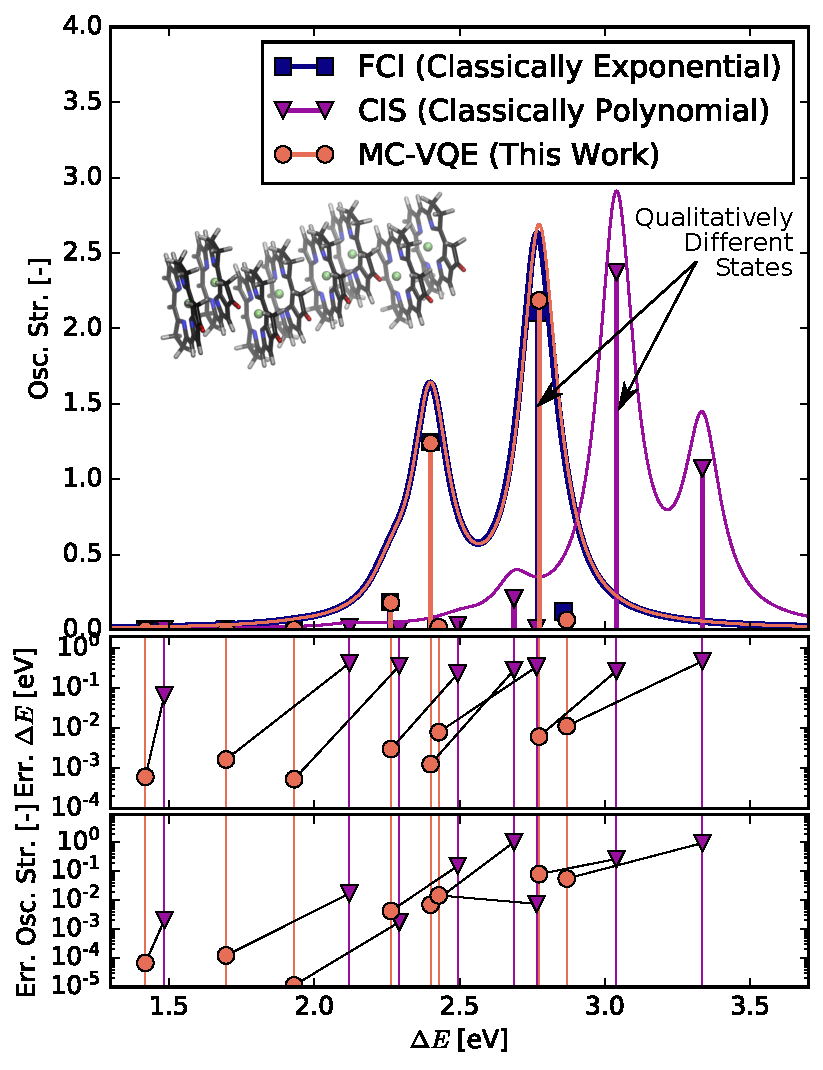
\includegraphics[width=3.2in]{stack2.pdf}
\caption{(color online). Top - Simulated absorption spectrum of $N=8$ linear
stack BChl-a test case (geometry depicted in inset), computed from the excitation
energies and oscillator strengths of the lowest 8 electronic transitions,
depicted as vertical sticks.  The envelope of the absorption spectrum is
sketched by broadening the contribution from each transition with a Lorentzian
with width of $\delta=0.15$ eV. The simulated MC-VQE and reference FCI results
are largely visually indistinguishable. Middle
- errors in excitation energies. Bottom - errors in oscillator strengths. Middle
  and bottom - thin lines are a guide for the eye.
}
\label{fig:stack}
\end{center}
\end{figure}

% \bibliography{jrncodes.bib,refs.bib}
% \bibliographystyle{aip}

% ***** Figures and Tables *****

% \end{document}
%
% ****** End of file template.aps ******
